% slides.tex
\documentclass[20pt]{beamer}
\usepackage{listings}
\usepackage[utf8]{inputenc}
\usepackage{color}
\usepackage{graphicx}

\usetheme{default}
\usecolortheme{dove}
\useoutertheme{default}

% Slightly smaller title
\setbeamerfont{frametitle}{size=\large}
\setbeamerfont{verb}{size=\small}

% Font
\renewcommand{\ttdefault}{pcr}

% lst settings
\lstset{
    basicstyle=\ttfamily\small,
    gobble=4,
    keywordstyle=\ttfamily\bfseries,
    language=Haskell
}

\newcommand{\vspaced}{
    \vspace{5mm}
}

\begin{document}

\title{\texttt{tsuruCapital :: \\
    Lambda -> Dollar}}
\subtitle{FLP 2012}
\author{Jasper Van der Jeugt}
\date{December 12, 2012}

\begin{frame}[plain]
    \titlepage
\end{frame}

% Introduction
% ------------

\begin{frame}{Hello!}
    My name is Jasper \\
    Student at UGent \\
    I write Haskell \\
    Tsuru Capital \\
    \texttt{@jaspervdj} \\
    \texttt{jaspervdj.be}
    \begin{picture}(0.0, 0.0)
    \put(30.0, -35.0){
        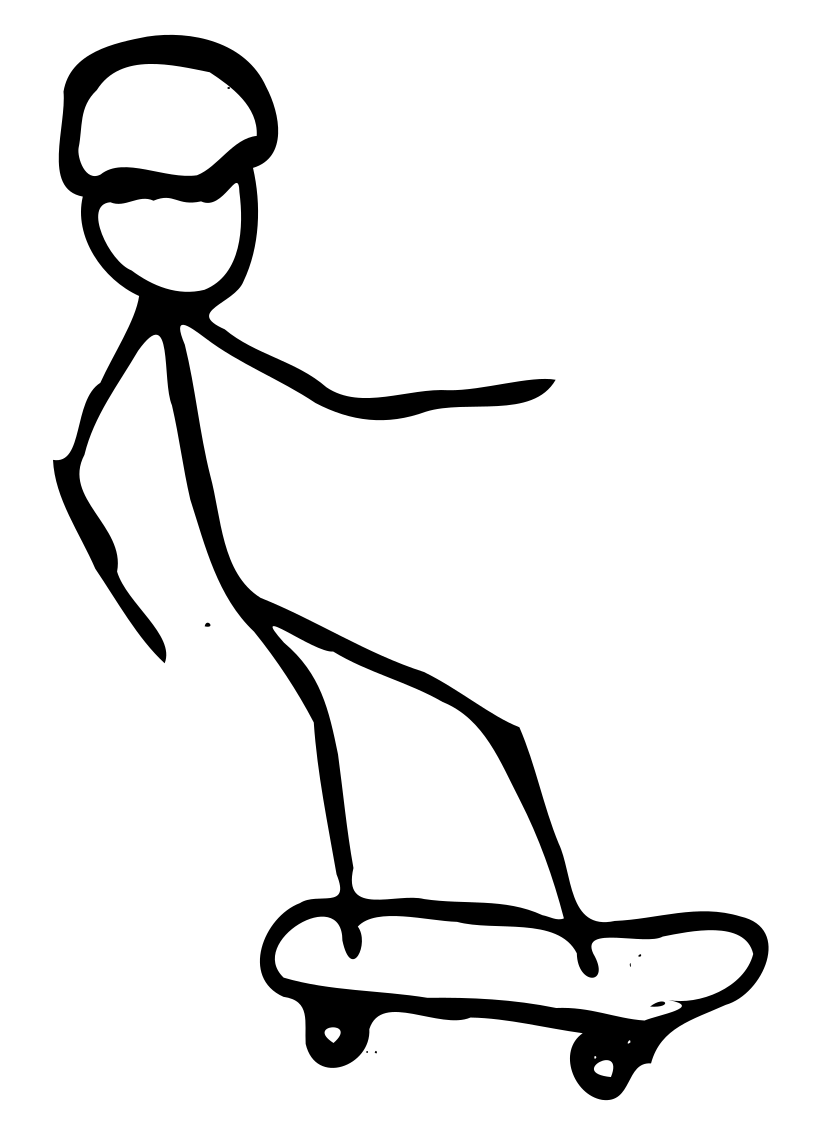
\includegraphics[width=0.5\textwidth]
            {../2012-ghentfpg-parallel/images/skate.pdf}}
    \end{picture}
\end{frame}

% About Tsuru Capital
% -------------------

\begin{frame}{Overview}
    \textbf{About Tsuru Capital} \\
    % TODO
\end{frame}

\begin{frame}{About Tsuru Capital}
    Privately held \\
    Finance \\
    Small team \\
    In-house software \\
\end{frame}

% Why Haskell
% -----------

\begin{frame}{Overview}
    % TODO
\end{frame}

\begin{frame}{Why Haskell?}
    \large{Why not Haskell?}
\end{frame}

\begin{frame}
    ``I don't know how we would possibly get anything done
    \emph{without} Haskell'' --- Alex
\end{frame}

\begin{frame}{Why Haskell?}
    First commit in 2008 \\
    Trader \& tools: $\pm$72k lines of Haskell \\
    Still some Bash scripts, some Ruby \\
    \vspaced
    (Not counting external libraries) \\
\end{frame}

\begin{frame}[fragile]{Why Haskell?}
    \textbf{Types} \\
    \vspaced
    \begin{lstlisting}
    newtype Price = P Int
    \end{lstlisting}
\end{frame}

\begin{frame}[fragile]{Why Haskell}
    \textbf{Types} \\
    \vspaced
    AveragePrice, FairPrice, KeyPrice, LikelyPrice, Price, StrikePrice,
    SynPrice...
\end{frame}

\begin{frame}[fragile]{Why Haskell}
    \textbf{Types} \\
    \vspaced
    Change the type of one function, \\
    break the entire build (yay!) \\
\end{frame}

% Example: parsers
% ----------------

\begin{frame}{Overview}
    % TODO
\end{frame}

\begin{frame}{Example: parsers}
    We write \emph{a lot} of parsers at Tsuru
\end{frame}

\begin{frame}{Example: parsers}
    \textbf{Parsers in Haskell} \\
    \vspaced
    Happy \\
    Parsec \\
    Attoparsec \\
    ... \\
\end{frame}

\begin{frame}[fragile]{Example: parsers}
    Typical proprietary packet \\
    \vspaced
    \begin{lstlisting}
    1 * 11 byte message no
    1 * 11 byte transaction code
    1 * 10 byte market opgroup code
    2 *  6 byte issue code
    5 * 12 byte best prices
    ...
    \end{lstlisting}
\end{frame}

\begin{frame}[fragile]{Example: parsers}
    Typically ASCII-only packets
    \vspaced
    \begin{lstlisting}
    KSEBID_0123011101100105...
    \end{lstlisting}
\end{frame}

\begin{frame}[fragile]{Example: parsers}
    Using e.g. Parsec \\
    \vspaced
    \begin{lstlisting}
    packet :: Parser Packet
    packet = do
        messageNo <- decimal 11
        transCode <- string 11
        opGroup   <- marketOpgroup
        ...
    \end{lstlisting}
\end{frame}

\begin{frame}{Example: parsers}
    New library: \textbf{Parsergen} \\
    \vspaced
    On github: \\
    \texttt{tsurucapital/parsergen}
\end{frame}

\begin{frame}[fragile]{Example: parsers}
    In Haskell... \\
    \vspaced
    \begin{lstlisting}
    newtype Volume = V Int
    newtype Price = P Int

    data Issuer = ...

    issuer :: Parser Issuer
    issuer = ...
    \end{lstlisting}
\end{frame}

\begin{frame}[fragile]{Example: parsers}
    In a separate file...
    \vspaced
    \begin{lstlisting}
    Packet
     Offer
      _Header   ByteString 3 "OFF"
      Issuer    Issuer     6 issuer
      5x Amount Volume     6
      5x Price  Price      6
    \end{lstlisting}
\end{frame}

\begin{frame}[fragile]{Example: parsers}
    In Haskell again... \\
    \vspaced
    \begin{lstlisting}
    $(genDataTypeFromFile
        "Packet.ths")
    $(genParserFromFile
        "Packet.ths")
    \end{lstlisting}
\end{frame}

\end{document}
